\documentclass[twoside,11pt]{article}

% Any additional packages needed should be included after jmlr2e.
% Note that jmlr2e.sty includes epsfig, amssymb, natbib and graphicx,
% and defines many common macros, such as 'proof' and 'example'.
%
% It also sets the bibliographystyle to plainnat; for more information on
% natbib citation styles, see the natbib documentation, a copy of which
% is archived at http://www.jmlr.org/format/natbib.pdf

% Available options for package jmlr2e are:
%
%   - abbrvbib : use abbrvnat for the bibliography style
%   - nohyperref : do not load the hyperref package
%   - preprint : remove JMLR specific information from the template,
%         useful for example for posting to preprint servers.
%
% Example of using the package with custom options:
%
% \usepackage[abbrvbib, preprint]{jmlr2e}
\usepackage[square,numbers]{natbib}
\bibliographystyle{plain}

\usepackage{jmlr2e}
\usepackage{graphicx}
\usepackage[ margin=1in]{geometry}
\usepackage{hyperref}
\hypersetup{colorlinks,linkcolor=blue,filecolor=blue,citecolor=magenta,urlcolor=blue}  

% Definitions of handy macros can go here

\newcommand{\dataset}{{\cal D}}
\newcommand{\fracpartial}[2]{\frac{\partial #1}{\partial  #2}}

% Heading arguments are {volume}{year}{pages}{date submitted}{date published}{paper id}{author-full-names}

%\jmlrheading{1}{2000}{1-48}{4/00}{10/00}{meila00a}{Marina Meil\u{a} and Michael I. Jordan}

% Short headings should be running head and authors last names
\usepackage{fancyhdr}%
\usepackage{lipsum}% Just for this example


\fancyhf{}% Clear all headers/footers
\fancyfoot[L]{}\fancyfoot[C]{Belhal Karimi, Research Statement}\fancyfoot[R]{}
\renewcommand{\headrulewidth}{0pt}
\pagestyle{fancy}
\rfoot{\thepage}
%\thispagestyle{plain}

%\ShortHeadings{Belhal Karimi, Research Statement}{Belhal Karimi, Research Statement}
\firstpageno{1}
\newlength\tindent
\setlength{\tindent}{\parindent}
\setlength{\parindent}{0pt}
\renewcommand{\indent}{\hspace*{\tindent}}
\renewcommand{\refname}{}
\usepackage[dvipsnames]{xcolor}
\definecolor{mygray}{gray}{0.3}


\begin{document}

%\title{Research Statement}
%
%\author{\name Belhal Karimi \email belhal.karimi@gmail.com \\
%       \addr Cognitive Computing Lab\
%       Baidu Research\\
%       Seattle, WA 98195-4322, USA}
%
%
%
%\maketitle
%
%\begin{abstract}%   <- trailing '%' for backward compatibility of .sty file
%...\end{abstract}
%
%\begin{keywords}
%...
%\end{keywords}
%
%\section{Introduction}


\textbf{\scalebox{2}{Research Statement}}  \hfill \textbf{\scalebox{1.5}{Belhal Karimi}} 

 \hfill \scalebox{1}{\textcolor{mygray}{\textsc{Baidu Research USA}}}

\hfill

Throughout my research, I focus on developing \emph{training}, also known as \emph{optimization}, methods for large-scale datasets.
There are several specificities to my work.

The broad panel of my work has applications on various problems, datasets and domains.
To name a few, such learning task as stated above is crucial while fitting complex nonlinear models (mixed models, deep neural networks, mixture models) on tabular, image, textual data to tackle problems encountered in computer vision, drug development or natural language processing.

Based on the principled approach that consists of \emph{observing} the world, \emph{designing} a model describing the best those observations and \emph{training} it on the latter, my main focal point in the realm of machine learning resides in the \emph{training}, or \emph{learning}, phase.
With the sheer size of data and the high nonconvexity of the modern models, such as mutlilayer nerual network, used to describe complex human tasks, there is a rising interest and need for scalable, faster learning methods and their rigorous theoretical understanding.

Up to some observations, either fixed or streaming, and a well designed model, the definition of a loss/cost function and its optimization (minimization) are at the heart of this training phase.
Continuously improving those optimization algorithms is key for \emph{machine learning} in order to sustain the rapid growth in dimension, compositionality of the models and the high variety of input observations (sound, image, LIDAR, etc \dots).

\begin{figure}[h]
\centering
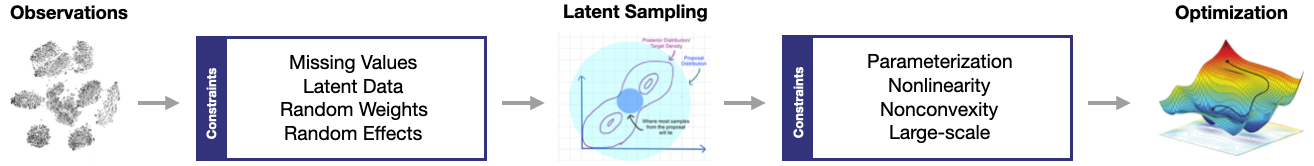
\includegraphics[width=\textwidth]{fig_summary}
%\caption{fhzuz}
%\label{fig:myresearch}
\end{figure}

While my work provides \emph{novel} methods for particularly deep neural networks (DNNs), one special case of the setting above, is when the input-output relationship of a phenomena is not completely characterized by the observations.
A set of latent variables is thus needed and the loss function accepts the latter as a third argument.

\textit{ Illustrative example of latent data model:} 
During clinical trials, the kinetics and dynamics of a drug being tested are modeled using nonlinear functions (or systems of ordinary differential equations) and observations from patients which comprise for instance their gender, height, the concentration of the drug after injection.
While those observed covariates are necessary, they are not sufficient to describe well the biological phenomena. 
A set of latent variables are used to quantify what can not be measured. 
In the special case of pharmacology, those latent variables describe the inter-individual variability among patients of a population (this is what makes us all different other than measurable signals). 
Therefore, the loss function, here the likelihood, is completed by simulations of those random effects and are then used to complete the observations before final optimization.

Thus, part of my research is at \emph{the intersection} of \textbf{sampling} and \textbf{optimization}, bridging the gap between sampling methods such as Markov Chain Monte Carlo (MCMC) or Variational Inference and optimization method such as gradient-based learning algorithms or maximum likelihood estimation.
My research has been published in top-tier conferences in machine learning such as NeurIPS, COLT, BAYSM, and made the object of contribution in statistics Journal such as CSDA. I also received a collection of awards from those conferences and a Jacques Hadamard grant for a summer visit to the Russian leading group in Bayesian Deep Learning called \emph{BayesGroup}.

%Some of my work is now implemented in the commercial modeling and simulation software for drug development \emph{Lixoft} and in its open-source counterpart \emph{saemix}.


\clearpage
%% ---------------------------------------------------Deep Learning: Training and Generalization-----------------------------------------------------------------------------------------
%\vspace{0.2in}
%\textbf{\scalebox{1.6}{(a) Deep Learning: Training and Generalization}}
%\vspace{0.2in}
%
%A particular interest of mine lies in the practical training and theoretical understanding of deep neural networks, widely used for most learning tasks in the past decade.
%Scaling, speeding, and improving existing training algorithms is of utmost importance and drive most of my existing publications.
%Recently, I have been also interested in the generalization properties of such training algorithms. 
%Speeding training and making sure the output parameter estimates lead to models generalizing well on unseen data are the two main challenges I am tackling today.
%
%\vspace{0.08in}
%\paragraph{Training Acceleration.} 
%Dealing with the speed of convergence of a given training algorithm is a classical problem in modern machine learning.
%From a theoretical perspective, we define the convergence of an algorithm when this latter reaches a so-called $\epsilon$-stationary point.
%In deep learning, and more generally in stochastic nonconvex optimization, the chosen suboptimality condition is the second order moment of the gradient of the objective function. 
%Then, deriving the algorithm convergence rate simply consists of finding the number of iterations until that quantity is bounded by $\epsilon$.
%In \citep{karimi2019non}, we  establish that the classical Stochastic Gradient Descent (SGD) algorithm reaches an $\epsilon$-stationary point in $\mathcal{O}\left(c_{0}+\log (n) / \sqrt{n}\right)$ iterations. 
%The results also hold when the stochastic gradient is biased, i.e., its expectation is not equal to the full gradient. 
%This setting has not been studied before our contribution and yet is presented in numerous applications such as the online EM algorithm or the policy-gradient method for reward maximization in reinforcement learning.
%
%From a practical perspective, we propose a variant of the known AMSGrad algorithm, a popular adaptive gradient method, in order to facilitate its acceleration.
%In \citep{kun2020}, we add prior knowledge about the sequence of consecutive mini-batch gradients and leverages its underlying structure making the gradients sequentially predictable. 
%By exploiting the predictability and ideas from optimistic online learning, our proposed algorithm accelerates the convergence and increases sample efficiency.
%In \citep{karimi2019misso}, we derive a unifying framework for incremental optimization methods. 
%Among others, our framework includes stochastic variational inference and MISO.
%
%\vspace{0.08in}
%\paragraph{Decentralized Training.} 
%Given the need for distributed training procedures, distributed optimization algorithms are at the center of attention. 
%With the growth of computing power and the need for using machine learning models on mobile devices, the communication cost of distributed training algorithms needs careful consideration. 
%In that regard, more and more attention is shifted from the traditional parameter server training paradigm to the decentralized one, which usually requires lower communication costs.
%We develop, in \citep{chen2020decent}, a general algorithmic framework that can convert existing adaptive gradient methods to their decentralized counterparts and thoroughly analyze the convergence behavior of the proposed algorithmic framework showing that if a given adaptive gradient method converges, under some specific conditions, then its decentralized counterpart is also convergent.
%
%Apart from the focus on communication complexity, the privacy of the data stored on the devices on which distributed learning occurs is also critical.
%In \citep{had2020}, we derive \textsc{FedSKETCH}, a method based on the compression of the accumulation of local gradients using count sketch.
%Due to the lower dimension of sketching used, our method exhibits communication-efficiency property. We also deal with the case where the data is heterogeneous across devices, which is commonly faced in federated learning, by developing \textsc{FedSKETCHGATE}.
%In particular, we establish a communication complexity of order $\mathcal{O}(\log(d))$ per round, where $d$ is the dimension of the vector of parameters compared to $\mathcal{O}(d)$ complexity per round of baseline mini-batch SGD.
%Another focus on the federated learning setting is made in our work \citep{karimi2020lars}, where we develop a local variant of AMSGrad by using layerwise and dimensionwise adaptive learning rates. The main contribution of the paper lies in the embedding of the LARS method in the local AMSGrad method.
%
%
%\vspace{0.08in}
%\paragraph{Towards Better Generalization.} 
%The final aspect of my work on training DNNs pertain to improving their generalization performances.
%Adaptive gradient methods have been optimizers of choice for deep learning due to their fast training speed, yet, their generalization performance is often worse than that of SGD for over-parameterized neural networks. 
%To tackle this flaw, we propose in \citep{zhou2020towards} Stable Adaptive Gradient Descent (\textsc{SAGD}) which leverages differential privacy to boost the generalization performance of adaptive gradient methods.
%Empirical runs on image classification or language modeling are backed with theoretical justifications to highlight the improved generalization properties of \textsc{SAGD}.
%
%
%
%\clearpage
%% ---------------------------------------------------When Sampling meets Optimization-----------------------------------------------------------------------------------------
%\vspace{0.2in}
%\textbf{\scalebox{1.6}{(b) When Sampling meets Optimization}}
%\vspace{0.2in}
%
%Mostly driven by the potential applications and as stated at the beginning of this statement, the models I am considering in my work are comprised of some latent variables.
%Indeed either in medical applications, where latent variables may be missing values uninformed by the patients or random effects in the special case of pharmacology, or in computer vision applications, and more specifically generative modeling, where layers of latent variables are used to disentangle a better representation of the input data, being able to \emph{sample/infer} those latent variables is key during the \emph{optimization} phase.
%I detail below different contributions where this setting is respected.
%
%%\vspace{0.15in}
%%\textbf{Fitting Latent Variable Models} 
%%\vspace{0.08in}
%\vspace{0.08in}
%\paragraph{Fitting Latent Variable Models.} 
%The EM algorithm is one of the most popular algorithm for maximum likelihood estimation in latent data models.
%We propose in \citep{karimi2019global}, a stochastic EM framework for exponential models encompassing incremental and several variance reduced variants.
%Our global and non-asymptotic bounds make the case for leveraging variance reduction techniques, borrowed from the optimization literature, to accelerate drastically the convergence to a stationary point taking $\mathcal{O}(n^{2/3}/\epsilon)$ for the latter versus $\mathcal{O}(n^/\epsilon)$ for the former, with $n$ being the number of data samples.
%From a modeling perspective, we propose in \citep{ren2020vfg} a novel approach to embed flow-based models with hierarchical latent data structures. 
%Integrating normalizing flows in variational graphs leads to a better recovery of the latent relational structures of high dimensional data.
%
%Moreover, a particularly interesting class of latent variable models is Bayesian Neural Networks (BNNs).
%BNNs attempt to combine the strong predictive performance of neural networks with formal quantification of uncertainty of the predicted output in the Bayesian framework.
%Yet, today, training those networks is slow and inefficient. 
%Thus, we propose in \citep{karimi2020hwa}, a simple averaging method in the space of the hyperparameters of the random weights leading to faster training and better empirical generalization.
%%Based on several heuristics and theoretical justifications from the literature, averaging snapshots of the models through the iterations is powerful while being very simple. 
%
%
%\vspace{0.08in}
%\paragraph{Two-level Stochastic Optimization Methods.} 
%The EM algorithm, when used on highly nonconvex models, is intractable.
%A natural solution is to alleviate the intractable expectations with Monte Carlo (MC) approximations.
%In \citep{karimi2019convergence} and \citep{karimi2020misso}, we analyze those variants when two levels of stochasticity are involved.
%The first one being the MC approximation and the second one the index sampling for stochastic updates.
%
%These works were followed by our Two-Timescale scheme in \citep{karimi2020tts}, where Robbins-Monro type of update is combined with stochastic variance reduction.
%Thus, two dynamics are progressing iteratively, one being driven by the stochastic approximation stepsize (slow) and the other one driven by the variance reduction stepsize (fast).
%Our framework displays better convergence performances for various applications from fitting pharmacological models to training deformable template for image analysis.
%
%\vspace{0.08in}
%\paragraph{MCMC Based Optimization.} 
%
%When MC approximation is involved, as stated above, sampling from the posterior distribution is not always direct.
%For complex models, we have recourse to sampling techniques such as VI or MCMC.
%We propose in \citep{karimi2017non, karimi2018eff} an efficient MCMC procedure, namely \textsc{nlme-IMH}, for posterior sampling in nonlinear mixed-effects models, based on the Laplace approximation.
%This work was followed by \citep{karimi2018fsaem} where we embed \textsc{nlme-IMH} into a stochastic variant of the EM algorithm (SAEM) for maximum likelihood estimation.
%
%In Energy Based Models (EBMs), this sampling procedure, aiming at drawing samples from the potential of the EBM, is crucial for the ultimate task of training a generative model.
%In \citep{karimi2020anila}, we improve current state-of-the-art samplers for EBMs by introducing an anisotropic stepsize in our Langevin updates.
%The drift term of the Langevin diffusion is not only depending on the dimension of the posterior landscape, but the covariance of the Brownian motion is also gradient informed. 
%Making the proposal empirically efficient to explore a larger space of the posterior distribution and thus avoiding in practice mode collapse.
%
%
%
%\clearpage
%% ---------------------------------------------------Distributed Optimization-----------------------------------------------------------------------------------------
%\vspace{0.2in}
%\textbf{\scalebox{1.6}{(c) Distributed Optimization}}
%\vspace{0.2in}
%
%
%\vspace{0.08in}
%\paragraph{Distributed Optimization Acceleration.} 
%
%
%\vspace{0.08in}
%\paragraph{Deep Federated Learning.} 
%
%
%
%\clearpage
%% ---------------------------------------------------Generative Modeling-----------------------------------------------------------------------------------------
%\vspace{0.2in}
%\textbf{\scalebox{1.6}{(d) Generative Modeling}}
%\vspace{0.2in}
%
%
%
%\vspace{0.08in}
%\paragraph{Improve the Sampling, improve the EBM.} 
%
%
%\vspace{0.08in}
%\paragraph{EBM and its Applications.} 
%
%
%
%\clearpage
%% ---------------------------------------------------Future Research Directions-----------------------------------------------------------------------------------------
%\vspace{0.25in}
%\textbf{\scalebox{1.6}{Future Research Directions}} 
%\vspace{0.15in}
%
%I would like to develop here the main axis of research I am planning on conducting in the next years, driven by the \emph{applications}, such as medical and vision, the power of \emph{Bayesian methods}, tools like \emph{MCMC} for posterior sampling and the leverage of a latent data structure considered as an additional layer on top of the observations. 
%I plan on leveraging all those latter techniques on the following tasks: training complex models under the federated settings when unobserved covariates (missing values, random effects, latent labels) are at stake, designing efficient sampling-based (MCMC or VI) optimization algorithms for training energy based models or bayesian neural networks, improving the understanding of generalization in over parametrized neural networks.
%
%\vspace{0.08in}
%\paragraph{Energy Based Models.} 
%EBMs are promising generative models particularly interesting to use in computer vision tasks.
%They are exactly at the crossroads of the sampling and the optimization domains.
%Developing efficient and clever MCMC proposals is key to greater exploration of the conditional distribution one needs to sample from and would lead to better mixing of the chain. 
%Especially when short-run MCMC is involved, the hyperparameters of the proposal distribution are crucial.
%Mode collapse is one of the challenges encountered and given the multimodal and nonconvex nature of the target distribution, several MCMC techniques, like the one we develop in \citep{karimi2020anila}, are worth considering.
%
%
%\vspace{0.08in}
%\paragraph{Federated Learning.} 
%Federated Learning has been a rapidly growing domain over the past years for its ability to handle data on million of devices while preserving their privacy.
%Our ability to come up with new communication efficient and private methods is utterly important in order to fit complex models, like DNNs, in order to describe human tasks in the decentralized settings.
%Before such progress is made, we will remain limited in the number of devices, data samples, and the nature of the tasks we can handle.
%\citep{had2020, karimi2020lars} were developed in that context.
%One other interesting direction, yet unexplored by the community, that I wish to contribute to is the study and adaptation of EM-like algorithms in the federated (decentralized and private) setting.
%More generally, latent variable models are not well studied under that setting and I believe that whenever latent inference is involved, a particular sampling procedure is needed in order to work under decentralized and private constraints.
%The natural and important application is the fitting on nonconvex models on hospital data where many data points are missing (thus considered as latent).
%
%
%\vspace{0.08in}
%\paragraph{Bayesian Deep Learning.} 
%In several sensible domains, such as medical or autonomous driving, being able to derive safety guarantees that \emph{take account of the uncertainty within the model and the input data} is mandatory before putting trained models in production.
%Bayesian deep learning, which assumes a prior over the weights, is capable of producing such uncertainty measures, yet their training and accuracy even on benchmark datasets are not satisfactory.
%In short, the current main issue I see is robustness, i.e., it should be as easy or easier to get to work than normal deep learning models, but it is not at the moment, and efficiency, i.e., it should at most be 2-3x as slow as normal deep learning training, but currently, it is slower.
%Developing optimization methods to tackle those challenges is important and will be one of my focus for the years to come.
%\citep{karimi2020hwa} and \citep{karimi2020misso} are attempts to give solutions to those issues.
%
%
%\vspace{0.08in}
%\paragraph{Generalization of Deep Neural Networks.} 
%While deep neural networks are working very well in practice, we have very little understanding of how they work. 
%Except working on improving the training and the generalization properties of those surprisingly well-performing over parametrized neural networks (as in our work  \citep{zhou2020towards}), focus needs to be put on explaining why they work so well on unseen data while their architectures contain more parameters than the number of training data points. 
%One possible direction towards that goal is to extensively understand the loss landscape that one is trying to minimize.
%Such knowledge is important to understand how the trajectory of the parameter estimates through the epochs, and hence \emph{a fortiori} the vector of fitted parameters, affect the generalization of our trained model.
%Some curvature, gradient and Hessian, based metrics are initial attempts at addressing those questions.
%For instance, we are developing a convergence diagnostic tool for nonconvex loss function (in particular DNNs) leveraging theoretical and empirical discoveries about stationarity metrics combined with sharpness and wideness of encountered local minima during the training procedure.
%Hopes are that combining saturation (widely used for convex functions) with generalization metrics, such that the curvature of the loss and the variance of the gradients, will lead to a convergence-based stepsize schedule favorable to better generalization.
%
%
%
%\clearpage
%% ---------------------------------------------------Conclusions-----------------------------------------------------------------------------------------
%
%\vspace{0.2in}
%\textbf{\scalebox{1.6}{Concluding Remarks}} 
%\vspace{0.2in}
%
%I am confident that my research and collaborations with experts in various fields, including machine learning, statistics, mathematics, and pharmacology have equipped me with the necessary background to approach the above challenging and impactful research directions.
%I believe the plan laid out above is coherent with my background, my skills, and most importantly my personal interests in contributing to the field.
%While those domains may seem highly diverse, I plan on contributing to each by providing novel \emph{optimization} and \emph{sampling} tools, as the core of my expertise.
%
%
%
%
%
%% ---------------------------------------------------References-----------------------------------------------------------------------------------------
%\newpage
%\textbf{\scalebox{1.6}{References}}
%\vspace{-0.3in}
%
%%\nocite{*}
%\bibliography{references}
%
\end{document}
